% Options for packages loaded elsewhere
\PassOptionsToPackage{unicode}{hyperref}
\PassOptionsToPackage{hyphens}{url}
%
\documentclass[10pt,twocolumn]{article}
\usepackage{amsmath,amssymb}
\usepackage{lmodern}
\usepackage{iftex}
\ifPDFTeX
  \usepackage[T1]{fontenc}
  \usepackage[utf8]{inputenc}
  \usepackage{textcomp} % provide euro and other symbols
\else % if luatex or xetex
  \usepackage{unicode-math}
  \defaultfontfeatures{Scale=MatchLowercase}
  \defaultfontfeatures[\rmfamily]{Ligatures=TeX,Scale=1}
\fi
% Use upquote if available, for straight quotes in verbatim environments
\IfFileExists{upquote.sty}{\usepackage{upquote}}{}
\IfFileExists{microtype.sty}{% use microtype if available
  \usepackage[]{microtype}
  \UseMicrotypeSet[protrusion]{basicmath} % disable protrusion for tt fonts
}{}
\makeatletter
\@ifundefined{KOMAClassName}{% if non-KOMA class
  \IfFileExists{parskip.sty}{%
    \usepackage{parskip}
  }{% else
    \setlength{\parindent}{0pt}
    \setlength{\parskip}{6pt plus 2pt minus 1pt}}
}{% if KOMA class
  \KOMAoptions{parskip=half}}
\makeatother
\usepackage{xcolor}
\IfFileExists{xurl.sty}{\usepackage{xurl}}{} % add URL line breaks if available
\IfFileExists{bookmark.sty}{\usepackage{bookmark}}{\usepackage{hyperref}}
\hypersetup{
  pdfauthor={Minmin Wu},
  hidelinks,
  pdfcreator={LaTeX via pandoc}}
\urlstyle{same} % disable monospaced font for URLs
\usepackage{color}
\usepackage{fancyvrb}
\newcommand{\VerbBar}{|}
\newcommand{\VERB}{\Verb[commandchars=\\\{\}]}
\DefineVerbatimEnvironment{Highlighting}{Verbatim}{
  commandchars=\\\{\},
  fontsize=\scriptsize
}
% Add ',fontsize=\small' for more characters per line
\newenvironment{Shaded}{}{}
\newcommand{\AlertTok}[1]{\textcolor[rgb]{1.00,0.00,0.00}{\textbf{#1}}}
\newcommand{\AnnotationTok}[1]{\textcolor[rgb]{0.38,0.63,0.69}{\textbf{\textit{#1}}}}
\newcommand{\AttributeTok}[1]{\textcolor[rgb]{0.49,0.56,0.16}{#1}}
\newcommand{\BaseNTok}[1]{\textcolor[rgb]{0.25,0.63,0.44}{#1}}
\newcommand{\BuiltInTok}[1]{#1}
\newcommand{\CharTok}[1]{\textcolor[rgb]{0.25,0.44,0.63}{#1}}
\newcommand{\CommentTok}[1]{\textcolor[rgb]{0.38,0.63,0.69}{\textit{#1}}}
\newcommand{\CommentVarTok}[1]{\textcolor[rgb]{0.38,0.63,0.69}{\textbf{\textit{#1}}}}
\newcommand{\ConstantTok}[1]{\textcolor[rgb]{0.53,0.00,0.00}{#1}}
\newcommand{\ControlFlowTok}[1]{\textcolor[rgb]{0.00,0.44,0.13}{\textbf{#1}}}
\newcommand{\DataTypeTok}[1]{\textcolor[rgb]{0.56,0.13,0.00}{#1}}
\newcommand{\DecValTok}[1]{\textcolor[rgb]{0.25,0.63,0.44}{#1}}
\newcommand{\DocumentationTok}[1]{\textcolor[rgb]{0.73,0.13,0.13}{\textit{#1}}}
\newcommand{\ErrorTok}[1]{\textcolor[rgb]{1.00,0.00,0.00}{\textbf{#1}}}
\newcommand{\ExtensionTok}[1]{#1}
\newcommand{\FloatTok}[1]{\textcolor[rgb]{0.25,0.63,0.44}{#1}}
\newcommand{\FunctionTok}[1]{\textcolor[rgb]{0.02,0.16,0.49}{#1}}
\newcommand{\ImportTok}[1]{#1}
\newcommand{\InformationTok}[1]{\textcolor[rgb]{0.38,0.63,0.69}{\textbf{\textit{#1}}}}
\newcommand{\KeywordTok}[1]{\textcolor[rgb]{0.00,0.44,0.13}{\textbf{#1}}}
\newcommand{\NormalTok}[1]{#1}
\newcommand{\OperatorTok}[1]{\textcolor[rgb]{0.40,0.40,0.40}{#1}}
\newcommand{\OtherTok}[1]{\textcolor[rgb]{0.00,0.44,0.13}{#1}}
\newcommand{\PreprocessorTok}[1]{\textcolor[rgb]{0.74,0.48,0.00}{#1}}
\newcommand{\RegionMarkerTok}[1]{#1}
\newcommand{\SpecialCharTok}[1]{\textcolor[rgb]{0.25,0.44,0.63}{#1}}
\newcommand{\SpecialStringTok}[1]{\textcolor[rgb]{0.73,0.40,0.53}{#1}}
\newcommand{\StringTok}[1]{\textcolor[rgb]{0.25,0.44,0.63}{#1}}
\newcommand{\VariableTok}[1]{\textcolor[rgb]{0.10,0.09,0.49}{#1}}
\newcommand{\VerbatimStringTok}[1]{\textcolor[rgb]{0.25,0.44,0.63}{#1}}
\newcommand{\WarningTok}[1]{\textcolor[rgb]{0.38,0.63,0.69}{\textbf{\textit{#1}}}}
\usepackage{longtable,booktabs,array}
\usepackage{tikz}
\usetikzlibrary{arrows.meta,positioning,shapes.geometric}
\newcounter{algorithm}
\usepackage{calc} % for calculating minipage widths
% Correct order of tables after \paragraph or \subparagraph
\usepackage{etoolbox}
\makeatletter
\patchcmd\longtable{\par}{\if@noskipsec\mbox{}\fi\par}{}{}
\makeatother
% Allow footnotes in longtable head/foot
\IfFileExists{footnotehyper.sty}{\usepackage{footnotehyper}}{\usepackage{footnote}}
\makesavenoteenv{longtable}
\setlength{\emergencystretch}{3em} % prevent overfull lines
\providecommand{\tightlist}{%
  \setlength{\itemsep}{0pt}\setlength{\parskip}{0pt}}
\setcounter{secnumdepth}{3}
\ifLuaTeX
  \usepackage{selnolig}  % disable illegal ligatures
\fi

\title{SessionBound: Turning Enterprise Task Approval into Budgeted
Database Sessions}
\author{Minmin Wu\\
Independent Researcher}
\date{}

\begin{document}

\twocolumn[
\begin{@twocolumnfalse}
\maketitle

\begin{abstract}

Enterprise AI agents are increasingly useful for internal analysis,
audit, compliance review, and operational investigation. They are good
at writing SQL on the fly, but enterprises cannot trust them with raw
database access. These tasks are typically approved above the database
layer by business users, managers, data owners, or compliance teams, but
executed below that layer through open-ended SQL generated by an agent.
This creates a missing systems layer: enterprise task approval must be
translated into a database execution context that is bounded, budgeted,
and auditable. SessionBound bridges this trust gap by turning a business
approval into a short-lived, budgeted, and auditable database session.

We present \textbf{SessionBound}, a control-plane and database-runtime
architecture that turns approved enterprise tasks into \textbf{budgeted
database sessions} for AI agents. A SessionBound control plane defines
task templates, accepts task applications, applies grants and approvals,
assigns TTLs and budgets, and issues signed task tokens. A database
runtime, \textbf{SessionBoundDB}, binds an approved task token to a
short-lived agent session and enforces safe views, row scope, denied
fields, operation limits, query budgets, disclosure budgets, and query
receipts at SQL execution time.

SessionBound does not require the database to parse natural-language
task descriptions, nor does it trust the agent or an LLM to correctly
interpret or obey the task. The agent remains free to generate SQL, join
safe business objects, aggregate, rank, and drill down. The database
decides whether each attempt stays inside the approved boundary. This
design targets a setting distinct from authenticated delegation,
task-scoped service-operation authorization, and data-product
marketplace access: enterprise-internal analytical work where fixed SaaS
screens are too rigid, direct database access is too broad, and approved
tasks should become temporary, budgeted, receipt-bearing database
sessions.

\textbf{Code availability.} The prototype source code, synthetic
evaluation dataset, validation reports, benchmark outputs, and arXiv
source are available at
\url{https://github.com/SessionBound/sessionbound}.
\end{abstract}

\vspace{1em}
\end{@twocolumnfalse}
]

\hypertarget{introduction}{%
\section{Introduction}\label{introduction}}

AI agents change how enterprise users interact with data. A user no
longer needs to know which report exists, which dashboard to open, or
which API endpoint to call. Instead, the user can ask an agent:

\begin{quote}
Analyze June 2026 travel reimbursements for the Sales department. Find
unusual merchants, repeated claims, employee-level monthly totals, and
claims near approval thresholds. Exclude salary and bank data.
\end{quote}

This is exactly the kind of task agents are good at: temporary,
exploratory, cross-table, and under-specified. It is also exactly the
kind of task traditional enterprise software handles poorly. Building a
permanent SaaS page or API for every low-frequency internal analysis
task is expensive. Giving the agent raw database access is unsafe.
Relying on prompts is not a security boundary. Relying on the
application layer alone becomes fragile when SQL is generated
dynamically.

The industry and research communities have already recognized several
adjacent problems. OAuth 2.0 provides the standard delegated
authorization model for web APIs~\cite{rfc6749}. Agent identity systems
make agents visible and governable as non-human identities.
Authenticated delegation frameworks let users verifiably delegate
authority to agents~\cite{south2025authenticateddelegation}.
Task-scoped authorization systems such as PAuth ask whether a specific
API or tool operation is implied by the user's
task~\cite{sharma2026pauth}. Data-product governance systems such as
Data Product MCP connect enterprise data marketplaces with MCP so that
agents can discover, request access to, and query governed data
products~\cite{tonnarelli2026dataproductmcp,mcp2025specification}.
Database security systems such as Oracle Deep Data Security show that
fine-grained policies should be enforced close to the
data~\cite{oracle2026deepdatasecuritydocs,oracle2026deepdatasecuritybrief}.
Large-scale authorization systems such as Zanzibar show how
relationship-based permission checks can be made consistent and
global~\cite{pang2019zanzibar}.

These are necessary pieces, but they leave a gap for enterprise-internal
analytical agents. In real organizations, a manager or data owner does
not log into a database to write row-level policies for every agent
task. A business user applies for or delegates a task. A manager, data
owner, or compliance workflow approves it. A data platform has already
registered safe business views. A system must convert the approved task
into a structured execution boundary that the database can enforce,
while still allowing the agent to freely generate useful analytical SQL.

This paper argues for the following principle: business users approve
tasks, not database policies. Agents generate SQL, but databases enforce
the approved boundary.

SessionBound separates three concerns.

\begin{enumerate}
\def\labelenumi{\arabic{enumi}.}
\tightlist
\item
  \textbf{Task control plane.} Defines task templates, accepts task
  applications, evaluates grants and approvals, assigns budgets and
  TTLs, and signs task tokens.
\item
  \textbf{Agent execution.} Lets an LLM-powered agent decide what SQL to
  try, which hypotheses to test, and how to construct a temporary
  workspace.
\item
  \textbf{Database runtime.} Binds the signed task token to a database
  session and enforces safe views, scope, denied fields, operation
  limits, query budgets, disclosure budgets, and receipts.
\end{enumerate}

The central design rule is that agents may explore only within a
structured boundary that the database enforces deterministically.

This makes SessionBound a contract layer between enterprise approval and
agentic database execution. The control plane records what the
organization approved; the runtime enforces how that approval may be
spent through SQL. This contract is not a database policy written by a
DBA, nor a natural-language instruction interpreted by an LLM. It is a
structured, signed, and accountable representation of an approved
business task that both the agent runtime and the database can interpret
deterministically.

SessionBoundDB is our PostgreSQL-based reference runtime for
SessionBound. It does not ask an LLM whether a query is safe. It does
not depend on the agent correctly interpreting the task. It does not
trust mutable session variables set by the agent. Instead, it validates
a signed task token, exposes only registered safe views, rejects raw
table access and denied fields, tracks query and disclosure budgets, and
records receipts for allowed and denied attempts.

The PostgreSQL prototype currently keeps the \texttt{taskbound} SQL
schema name for compatibility with the existing demo implementation.

\hypertarget{contributions}{%
\subsection{Contributions}\label{contributions}}

This paper makes five contributions.

\begin{enumerate}
\def\labelenumi{\arabic{enumi}.}
\item
  \textbf{Enterprise task approval as the missing layer.} We identify a
  gap between agent delegation and database enforcement: real
  enterprises approve tasks, scopes, and budgets above the database, but
  need those approvals translated into database-enforceable execution
  boundaries.
\item
  \textbf{SessionBound control plane.} We propose a task control plane
  with task templates, task applications, task approvals, grants, TTLs,
  budgets, and signed task tokens. This control plane lets business and
  data-governance workflows define what work is authorized without
  requiring managers to write database policies.
\item
  \textbf{Budgeted database sessions.} We define a database session
  model in which an approved task token binds an agent to safe views,
  row scope, denied fields, allowed operations, TTL, query budget,
  disclosure budget, and audit receipt policy.
\item
  \textbf{LLM-independent enforcement for open-ended SQL.}
  SessionBoundDB allows agents to generate SQL freely inside a boundary,
  but the database enforces that boundary deterministically. The
  database does not parse the natural-language task and does not rely on
  an LLM to judge safety at query time.
\item
  \textbf{PostgreSQL prototype and hardening analysis.} We implement
  SessionBoundDB as a PostgreSQL-based runtime for SessionBound and
  demonstrate it on enterprise travel reimbursement analysis. We also
  analyze anti-evasion scope, budget semantics, schema drift,
  credential-token binding, receipt structure, and
  prototype-to-production hardening requirements.
\end{enumerate}


\hypertarget{motivation-enterprise-tasks-are-approved-above-the-database}{%
\section{Motivation: Enterprise Tasks Are Approved Above the
Database}\label{motivation-enterprise-tasks-are-approved-above-the-database}}

\hypertarget{saas-is-strong-at-fixed-workflows-and-weak-at-temporary-analysis}{%
\subsection{SaaS is strong at fixed workflows and weak at
temporary
analysis}\label{saas-is-strong-at-fixed-workflows-and-weak-at-temporary-analysis}}

Traditional SaaS applications are excellent for stable workflows.
Expense systems have pages for submitting claims, approving them, and
exporting reports. CRM systems have pages for accounts, opportunities,
and pipeline forecasts. HR systems have forms for updating employee
details. These interfaces are valuable because they encode product
experience, business rules, and human responsibility.

But enterprises also contain many tasks that are temporary, analytical,
and low-frequency:

\begin{itemize}
\tightlist
\item
  audit unusual reimbursement patterns for one month;
\item
  compare vendor concentration across departments;
\item
  investigate repeated support escalations for a customer segment;
\item
  find transactions near policy thresholds;
\item
  review access logs for a compliance incident;
\item
  build a temporary workspace for a manager's operational question.
\end{itemize}

These tasks are too specific to justify permanent SaaS pages, but too
sensitive to give an agent raw database access. They often require
joins, aggregation, ranking, drill-down, and follow-up queries. The
exact SQL cannot be known in advance.

SessionBound targets this setting.

\hypertarget{enterprise-approval-is-not-database-policy-authoring}{%
\subsection{Enterprise approval is not database policy
authoring}\label{enterprise-approval-is-not-database-policy-authoring}}

In a realistic enterprise, a manager or data owner should not be
expected to write SQL policies. A business user might request:

\begin{quote}
\begin{description}
\tightlist
\item[Task type:]
{\scriptsize\texttt{monthly\_expense\_anomaly\_review}}
\item[Scope:]
June 2026, Sales department
\item[Purpose:]
travel reimbursement audit
\item[Sensitivity:]
exclude salary, phone, bank account
\item[Budget:]
up to 20 SQL attempts, 5,000 result rows, and limited entity exposure
\item[TTL:]
30 minutes
\end{description}
\end{quote}

A manager or data owner can decide whether this task is appropriate. A
data platform can provide approved safe views. A compliance system can
require tighter budgets. But none of these people should need to edit
database roles, row-level security predicates, or cell-level policies
for every agent session.

SessionBound therefore separates task governance from database
enforcement:

\begin{verbatim}
Business users approve tasks.
Data platforms register safe views.
Control planes sign task tokens.
Databases enforce boundaries.
Agents explore freely inside
those boundaries.
\end{verbatim}

\hypertarget{running-example-travel-reimbursement-anomaly-review}{%
\subsection{Running example: travel reimbursement anomaly
review}\label{running-example-travel-reimbursement-anomaly-review}}

We use travel reimbursement review as a running example. A finance
analyst or department manager wants an agent to analyze June travel
reimbursements for a department. The agent may need to:

\begin{itemize}
\tightlist
\item
  rank high-value claims;
\item
  group expenses by merchant, city, category, and employee;
\item
  compute monthly employee totals;
\item
  find claims close to approval thresholds;
\item
  drill down into suspicious patterns;
\item
  propose follow-up review actions.
\end{itemize}

The agent should not see salary, bank account, phone number, or raw
internal tables. It should not query another department, another month,
or another tenant. It should not run DDL or arbitrary updates. It should
not paginate through all employees and reconstruct an unrestricted
dataset. Its access should expire quickly and leave an audit trail.

A fixed API such as \texttt{get\_expense\_summary(department,\ month)}
is too narrow. A broad database account is too dangerous. A prompt
instruction such as ``do not access salary'' is not a security
mechanism. SessionBound's answer is to approve a task and bind it to a
database session with safe views, scope, budgets, and receipts.


\hypertarget{threat-model}{%
\section{Threat Model}\label{threat-model}}

SessionBound assumes the upper-layer agent is useful but not trusted.
The agent may be confused, overconfident, prompt-injected, malicious, or
simply wrong. The database boundary must remain meaningful even when the
agent tries the wrong thing.

\hypertarget{trusted-components}{%
\subsection{Trusted components}\label{trusted-components}}

For this prototype, we trust:

\begin{itemize}
\tightlist
\item
  the task control plane that defines templates, evaluates grants,
  records approvals, and signs task tokens;
\item
  the credential broker that issues short-lived database credentials;
\item
  the database runtime that validates tokens and enforces policies;
\item
  the cryptographic signing key or signing service used for task tokens;
\item
  the integrity of registered safe views and runtime functions.
\end{itemize}

In production, the signing path should be backed by a KMS, JWKS,
hardware-backed key service, or enterprise identity infrastructure. The
prototype uses a simpler signing path for demonstration.

\hypertarget{untrusted-or-partially-trusted-components}{%
\subsection{Untrusted or partially trusted
components}\label{untrusted-or-partially-trusted-components}}

We do not trust:

\begin{itemize}
\tightlist
\item
  the agent's prompt;
\item
  the agent's reasoning;
\item
  the agent's SQL generation;
\item
  the agent's natural-language interpretation of the task;
\item
  user-provided or database-provided text that may contain prompt
  injection;
\item
  ordinary client-controlled session variables;
\item
  application-layer filtering as the final boundary.
\end{itemize}

This is the main difference from designs that require an LLM to infer
the precise intended operation from natural language. SessionBound does
not ask the database to understand the user's natural-language intent.
The database consumes structured claims from a signed token.

\hypertarget{in-scope-threats}{%
\subsection{In-scope threats}\label{in-scope-threats}}

SessionBoundDB is designed to mitigate:

\begin{itemize}
\tightlist
\item
  \textbf{Sensitive field access}: attempts to read salary, bank
  account, phone, identity number, credentials, or private notes.
\item
  \textbf{Raw table access}: attempts to bypass safe views and query
  application schemas directly.
\item
  \textbf{Scope escape}: attempts to read other tenants, months,
  departments, projects, or users.
\item
  \textbf{Unauthorized mutations}: attempts to run \texttt{INSERT},
  \texttt{UPDATE}, \texttt{DELETE}, DDL, or high-impact operations
  outside controlled commands.
\item
  \textbf{Prompt injection effects}: data or user text instructs the
  agent to ignore policy or reveal secrets.
\item
  \textbf{Budget evasion}: repeated queries, pagination, or alternate
  SQL forms attempt to disclose more detail rows than the task allows.
\item
  \textbf{Credential-token mismatch}: attempts to combine one runtime
  credential with another task token.
\end{itemize}

\hypertarget{out-of-scope}{%
\subsection{Out of scope}\label{out-of-scope}}

The prototype does not solve:

\begin{itemize}
\tightlist
\item
  malicious database administrators;
\item
  compromised database host operating systems;
\item
  compromised signing infrastructure;
\item
  side-channel attacks;
\item
  complete formal verification of SQL equivalence;
\item
  production-grade SQL AST enforcement;
\item
  cross-database federation;
\item
  full differential privacy for statistical releases;
\item
  arbitrary semantic inference across all allowed query answers.
\end{itemize}

SessionBound reduces and accounts for what an agent can discover. It
does not claim to eliminate all inference.


\hypertarget{sessionbound-model}{%
\section{SessionBound Model}\label{sessionbound-model}}

SessionBound has two major layers: a task control plane and a database
runtime. Figure~\ref{fig:sessionbound-architecture} shows the main
SessionBound control-plane and runtime boundary.

\begin{figure*}[t]
\centering
\resizebox{0.92\textwidth}{!}{%
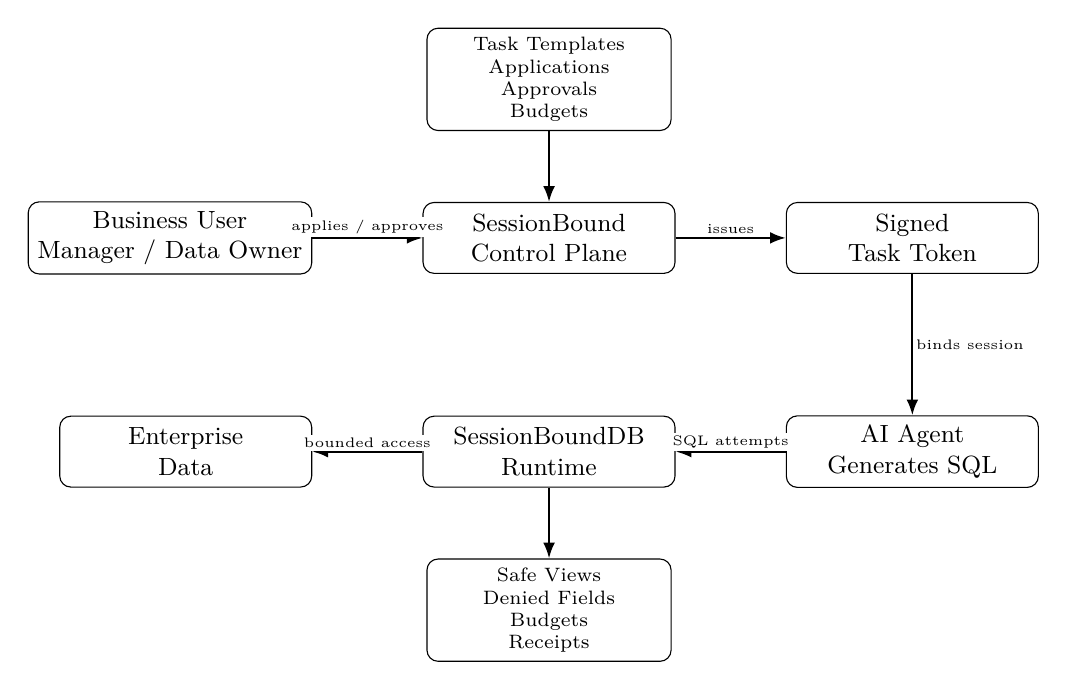
\begin{tikzpicture}[
  node distance=9mm and 14mm,
  box/.style={
    draw,
    rounded corners,
    align=center,
    minimum width=32mm,
    minimum height=9mm,
    font=\small
  },
  smallbox/.style={
    draw,
    rounded corners,
    align=center,
    minimum width=31mm,
    minimum height=8mm,
    font=\scriptsize
  },
  arrow/.style={-{Latex[length=2mm]}, thick},
  edgelabel/.style={font=\tiny, fill=white, inner sep=1pt}
]
\node[box] (business) {Business User\\Manager / Data Owner};
\node[box, right=of business] (control) {SessionBound\\Control Plane};
\node[box, right=of control] (token) {Signed\\Task Token};

\node[smallbox, above=of control] (template) {Task Templates\\Applications\\Approvals\\Budgets};

\node[box, below=18mm of control] (runtime) {SessionBoundDB\\Runtime};
\node[box, left=of runtime] (data) {Enterprise\\Data};
\node[box, right=of runtime] (agent) {AI Agent\\Generates SQL};

\node[smallbox, below=of runtime] (enforce) {Safe Views\\Denied Fields\\Budgets\\Receipts};

\draw[arrow] (business) -- node[above, edgelabel]{applies / approves} (control);
\draw[arrow] (control) -- node[above, edgelabel]{issues} (token);
\draw[arrow] (token) -- node[right, edgelabel]{binds session} (agent);
\draw[arrow] (agent) -- node[above, edgelabel]{SQL attempts} (runtime);
\draw[arrow] (runtime) -- node[above, edgelabel]{bounded access} (data);
\draw[arrow] (template) -- (control);
\draw[arrow] (runtime) -- (enforce);
\end{tikzpicture}
}
\caption{SessionBound architecture. The control plane turns enterprise task approval into a signed task token; the agent may generate SQL freely, but SessionBoundDB enforces safe views, denied fields, budgets, and receipts inside the database session.}
\label{fig:sessionbound-architecture}
\end{figure*}

\hypertarget{task-template}{%
\subsection{Task template}\label{task-template}}

A task template is defined by a data platform or application team. It
describes a class of work that can be safely delegated to agents once
scoped and approved.

Example:

\begin{Shaded}
\begin{Highlighting}[]
\FunctionTok{\{}
  \DataTypeTok{"task\_type"}\FunctionTok{:} \StringTok{"monthly\_expense\_anomaly\_review"}\FunctionTok{,}
  \DataTypeTok{"purpose"}\FunctionTok{:} \StringTok{"travel\_reimbursement\_audit"}\FunctionTok{,}
  \DataTypeTok{"allowed\_views"}\FunctionTok{:} \OtherTok{[}\StringTok{"expenses"}\OtherTok{,} \StringTok{"employees"}\OtherTok{,} \StringTok{"departments"}\OtherTok{]}\FunctionTok{,}
  \DataTypeTok{"denied\_columns"}\FunctionTok{:} \OtherTok{[}
    \StringTok{"employees.salary"}\OtherTok{,}
    \StringTok{"employees.bank\_account"}\OtherTok{,}
    \StringTok{"employees.phone"}
  \OtherTok{]}\FunctionTok{,}
  \DataTypeTok{"required\_scope"}\FunctionTok{:} \OtherTok{[}\StringTok{"tenant\_id"}\OtherTok{,} \StringTok{"expense\_month"}\OtherTok{,} \StringTok{"department\_id"}\OtherTok{]}\FunctionTok{,}
  \DataTypeTok{"allowed\_operations"}\FunctionTok{:} \OtherTok{[}\StringTok{"SELECT"}\OtherTok{]}\FunctionTok{,}
  \DataTypeTok{"default\_ttl\_minutes"}\FunctionTok{:} \DecValTok{30}\FunctionTok{,}
  \DataTypeTok{"default\_budget"}\FunctionTok{:} \FunctionTok{\{}
    \DataTypeTok{"max\_queries"}\FunctionTok{:} \DecValTok{20}\FunctionTok{,}
    \DataTypeTok{"max\_result\_rows"}\FunctionTok{:} \DecValTok{5000}\FunctionTok{,}
    \DataTypeTok{"max\_unique\_entities"}\FunctionTok{:} \FunctionTok{\{}
      \DataTypeTok{"expense\_id"}\FunctionTok{:} \DecValTok{5000}\FunctionTok{,}
      \DataTypeTok{"employee\_id"}\FunctionTok{:} \DecValTok{200}
    \FunctionTok{\}}
  \FunctionTok{\}}
\FunctionTok{\}}
\end{Highlighting}
\end{Shaded}

The template is not generated by the agent. It is part of enterprise
governance.

\hypertarget{task-application}{%
\subsection{Task application}\label{task-application}}

A task application is a concrete request to perform work under a
template.

\begin{Shaded}
\begin{Highlighting}[]
\FunctionTok{\{}
  \DataTypeTok{"task\_type"}\FunctionTok{:} \StringTok{"monthly\_expense\_anomaly\_review"}\FunctionTok{,}
  \DataTypeTok{"requested\_by"}\FunctionTok{:} \StringTok{"user:alice"}\FunctionTok{,}
  \DataTypeTok{"actor"}\FunctionTok{:} \StringTok{"agent:travel{-}expense{-}analyst"}\FunctionTok{,}
  \DataTypeTok{"scope"}\FunctionTok{:} \FunctionTok{\{}
    \DataTypeTok{"tenant\_id"}\FunctionTok{:} \StringTok{"company\_a"}\FunctionTok{,}
    \DataTypeTok{"expense\_month"}\FunctionTok{:} \StringTok{"2026{-}06"}\FunctionTok{,}
    \DataTypeTok{"department\_id"}\FunctionTok{:} \StringTok{"dep\_sales"}
  \FunctionTok{\},}
  \DataTypeTok{"reason"}\FunctionTok{:} \StringTok{"Review unusual travel reimbursement patterns."}
\FunctionTok{\}}
\end{Highlighting}
\end{Shaded}

\hypertarget{task-approval}{%
\subsection{Task approval}\label{task-approval}}

A task approval evaluates whether the requester may run this task with
this scope and budget. Approval may be automatic, role-based, or manual.
For sensitive tasks, a manager, data owner, or compliance reviewer may
approve it.

The approval does not require the approver to write SQL policies. It
decides whether this scoped task should exist.

\hypertarget{task-token}{%
\subsection{Task token}\label{task-token}}

A signed task token is the structured authorization object consumed by
the database runtime.

\begin{Shaded}
\begin{Highlighting}[]
\FunctionTok{\{}
  \DataTypeTok{"task\_id"}\FunctionTok{:} \StringTok{"task\_456"}\FunctionTok{,}
  \DataTypeTok{"task\_type"}\FunctionTok{:} \StringTok{"monthly\_expense\_anomaly\_review"}\FunctionTok{,}
  \DataTypeTok{"delegator"}\FunctionTok{:} \StringTok{"user:alice"}\FunctionTok{,}
  \DataTypeTok{"actor"}\FunctionTok{:} \StringTok{"agent:travel{-}expense{-}analyst"}\FunctionTok{,}
  \DataTypeTok{"credential\_id"}\FunctionTok{:} \StringTok{"cred\_123"}\FunctionTok{,}
  \DataTypeTok{"tenant\_id"}\FunctionTok{:} \StringTok{"company\_a"}\FunctionTok{,}
  \DataTypeTok{"purpose"}\FunctionTok{:} \StringTok{"travel\_reimbursement\_audit"}\FunctionTok{,}
  \DataTypeTok{"allowed\_views"}\FunctionTok{:} \OtherTok{[}\StringTok{"expenses"}\OtherTok{,} \StringTok{"employees"}\OtherTok{,} \StringTok{"departments"}\OtherTok{]}\FunctionTok{,}
  \DataTypeTok{"denied\_columns"}\FunctionTok{:} \OtherTok{[}
    \StringTok{"employees.salary"}\OtherTok{,}
    \StringTok{"employees.bank\_account"}\OtherTok{,}
    \StringTok{"employees.phone"}
  \OtherTok{]}\FunctionTok{,}
  \DataTypeTok{"row\_scope"}\FunctionTok{:} \FunctionTok{\{}
    \DataTypeTok{"expense\_month"}\FunctionTok{:} \StringTok{"2026{-}06"}\FunctionTok{,}
    \DataTypeTok{"department\_id"}\FunctionTok{:} \StringTok{"dep\_sales"}
  \FunctionTok{\},}
  \DataTypeTok{"operations"}\FunctionTok{:} \OtherTok{[}\StringTok{"SELECT"}\OtherTok{]}\FunctionTok{,}
  \DataTypeTok{"budget"}\FunctionTok{:} \FunctionTok{\{}
    \DataTypeTok{"max\_queries"}\FunctionTok{:} \DecValTok{20}\FunctionTok{,}
    \DataTypeTok{"max\_result\_rows"}\FunctionTok{:} \DecValTok{5000}\FunctionTok{,}
    \DataTypeTok{"max\_unique\_entities"}\FunctionTok{:} \FunctionTok{\{}
      \DataTypeTok{"expense\_id"}\FunctionTok{:} \DecValTok{5000}\FunctionTok{,}
      \DataTypeTok{"employee\_id"}\FunctionTok{:} \DecValTok{200}
    \FunctionTok{\}}
  \FunctionTok{\},}
  \DataTypeTok{"safe\_view\_registry\_version"}\FunctionTok{:} \StringTok{"travel{-}demo{-}v1"}\FunctionTok{,}
  \DataTypeTok{"policy\_version"}\FunctionTok{:} \StringTok{"expense{-}review{-}v1"}\FunctionTok{,}
  \DataTypeTok{"audience"}\FunctionTok{:} \StringTok{"taskbounddb"}\FunctionTok{,}
  \DataTypeTok{"expires\_at"}\FunctionTok{:} \StringTok{"2026{-}06{-}24T10:30:00Z"}\FunctionTok{,}
  \DataTypeTok{"nonce"}\FunctionTok{:} \StringTok{"..."}
\FunctionTok{\}}
\end{Highlighting}
\end{Shaded}

\hypertarget{budgeted-database-session}{%
\subsection{Budgeted database
session}\label{budgeted-database-session}}

A budgeted database session is a database session bound to one active
task token. The session may issue open-ended SQL, but every attempt is
checked against the token, safe view registry, operation policy, and
remaining budget.

A connection may bind at most one active task token. Rebinding is
denied. When the token expires or is revoked, further
\texttt{taskbound.run} calls fail.


\hypertarget{control-plane-templates-applications-approvals-and-budgets}{%
\section{Control Plane: Templates, Applications, Approvals, and
Budgets}\label{control-plane-templates-applications-approvals-and-budgets}}

The control plane is the SaaS-like layer that makes SessionBound
realistic for enterprises. This is where SessionBound differs most
clearly from database-only security systems.

\hypertarget{business-users-approve-tasks-not-policies}{%
\subsection{Business users approve tasks, not
policies}\label{business-users-approve-tasks-not-policies}}

A data owner should see:

\begin{verbatim}
Alice requests a June Sales
travel reimbursement anomaly review.
Scope: Sales department, June 2026.
Denied: salary, bank account, phone.
Budget: 20 queries, bounded
entity exposure.
TTL: 30 minutes.
\end{verbatim}

The data owner should not see:

\begin{Shaded}
\begin{Highlighting}[]
\KeywordTok{CREATE}\NormalTok{ POLICY }\OperatorTok{..}\NormalTok{.}
\KeywordTok{ALTER} \KeywordTok{ROLE} \OperatorTok{..}\NormalTok{.}
\KeywordTok{GRANT} \KeywordTok{SELECT} \KeywordTok{ON} \OperatorTok{..}\NormalTok{.}
\end{Highlighting}
\end{Shaded}

The control plane converts the business approval into a signed token
that the runtime can enforce.

\hypertarget{grants-and-eligibility}{%
\subsection{Grants and
eligibility}\label{grants-and-eligibility}}

Roles do not grant direct database access. They grant eligibility to
request task templates. For example, a finance reviewer may be eligible
to request finance-review tasks; a department manager may be eligible to
request department-scoped analysis tasks.

This avoids broad database roles such as:

\begin{verbatim}
finance_user can access all finance tables
\end{verbatim}

Instead, the database sees a concrete task token: agent X may analyze
June 2026 Sales reimbursements using views A, B, C under budget Y.

\hypertarget{budget-assignment}{%
\subsection{Budget assignment}\label{budget-assignment}}

Budget assignment is a control-plane decision. A low-risk task might
receive a larger aggregate budget; a sensitive task may receive a small
detail-row budget and a short TTL. Budgets can be adjusted by role, data
classification, task purpose, and approval route.

The database runtime enforces the budget; the control plane decides what
budget is appropriate.


\hypertarget{sessionbounddb-runtime}{%
\section{SessionBoundDB Runtime}\label{sessionbounddb-runtime}}

SessionBoundDB is the PostgreSQL-based database runtime for
SessionBound.

\hypertarget{session-binding-and-credential-token-binding}{%
\subsection{Session binding and credential-token
binding}\label{session-binding-and-credential-token-binding}}

The runtime begins with two objects:

\begin{enumerate}
\def\labelenumi{\arabic{enumi}.}
\tightlist
\item
  a short-lived database credential issued by the credential broker;
\item
  a signed task token issued by the control plane.
\end{enumerate}

The credential authenticates the runtime connection. The task token
authorizes the work.

At \texttt{bind\_task}, the runtime checks:

\begin{itemize}
\tightlist
\item
  the task token signature is valid;
\item
  the task token is unexpired and not revoked;
\item
  the credential is unexpired and not revoked;
\item
  the token \texttt{credential\_id} matches the current session
  credential;
\item
  the token \texttt{actor} matches the credential actor;
\item
  the session login role matches the broker-issued database user;
\item
  the token audience is \texttt{taskbounddb};
\item
  no other active task is already bound to this database
  backend/session.
\end{itemize}

A stolen credential without a matching token is insufficient. A stolen
token without the matching credential is insufficient. Credential-token
binding reduces cross-task credential misuse.

PostgreSQL nuance: inside \texttt{SECURITY\ DEFINER} functions,
\texttt{current\_user} may refer to the function owner. Therefore, a
production implementation should use \texttt{session\_user} and/or an
explicit credential registry mapping rather than relying on
\texttt{current\_user} alone.

\hypertarget{safe-views-as-the-query-surface}{%
\subsection{Safe views as the query
surface}\label{safe-views-as-the-query-surface}}

Agents do not query raw application tables. They query registered safe
views. Safe views expose business objects, not internal schemas. This is
complementary to database-native mechanisms such as PostgreSQL
row-level security policies, which provide row filtering at the database
layer~\cite{postgresql2026rowsecurity}.

Example safe views:

\begin{verbatim}
expenses
employees
departments
approval_events
ledger_entries
\end{verbatim}

A safe view may:

\begin{itemize}
\tightlist
\item
  join raw tables into business objects;
\item
  remove sensitive fields;
\item
  apply tenant, department, month, or project scope;
\item
  expose workflow hints;
\item
  include stable business identifiers for budget accounting.
\end{itemize}

Safe views are not a complete inference-control solution. They reduce
the discoverable surface and make it governable.

\hypertarget{operation-policy}{%
\subsection{Operation policy}\label{operation-policy}}

\texttt{taskbound.run(sql)} is intended for read-only analytical SQL.
High-value writes should use controlled commands or stored procedures.
The runtime rejects mutations, DDL, unsafe utility commands, raw schema
access, denied fields, and blocked schemas.

\hypertarget{query-decision-pipeline}{%
\subsection{Query decision
pipeline}\label{query-decision-pipeline}}

At runtime, every SQL attempt follows the deterministic decision
procedure in Algorithm~\ref{alg:sql-decision-pipeline}.

\begin{center}
\refstepcounter{algorithm}\label{alg:sql-decision-pipeline}
\begin{minipage}{0.9\linewidth}
\textbf{Algorithm \thealgorithm. SQL decision pipeline for SessionBoundDB}

\textbf{Input:} SQL attempt and bound database session state.

\textbf{Output:} Allowed result with receipt, or denial receipt.

\begin{enumerate}
\item Require an active task binding for the session.
\item Validate the signed task token and its TTL.
\item Resolve all referenced relations against registered safe views.
\item Reject denied fields and blocked schemas.
\item Enforce row scope predicates for the bound task.
\item Reject disallowed operation types, including mutations, DDL, and
unsafe utility commands.
\item Check remaining query and disclosure budgets.
\item If every check passes, execute the query and emit an allow receipt;
otherwise reject the attempt and emit a denial receipt.
\end{enumerate}
\end{minipage}
\end{center}

The runtime does not ask an LLM whether a query is safe.


\hypertarget{anti-evasion-scope}{%
\section{Anti-Evasion Scope}\label{anti-evasion-scope}}

SessionBound handles direct boundary violations, but it does not claim
to eliminate all semantic inference attacks. This distinction is central
to the design.

\hypertarget{direct-boundary-violations}{%
\subsection{Direct boundary
violations}\label{direct-boundary-violations}}

SessionBoundDB can directly block:

\begin{itemize}
\tightlist
\item
  access to raw schemas;
\item
  access to sensitive fields that are not exposed through safe views;
\item
  queries outside row scope;
\item
  unsupported operation types;
\item
  repeated querying beyond task budgets;
\item
  use of credentials without a matching task token;
\item
  attempts to continue after token expiry or revocation.
\end{itemize}

\hypertarget{inference-and-side-channels}{%
\subsection{Inference and side
channels}\label{inference-and-side-channels}}

SessionBound does not claim to solve arbitrary inference from allowed
answers. For example, if a safe view exposes enough correlated
information, an agent may infer sensitive facts indirectly. Aggregates
over small groups may leak more than intended. Timing and resource side
channels are also outside the prototype's formal guarantees.
Classical database inference-control work studies these risks for
statistical databases and repeated query answers~\cite{adam1989securitycontrol}.

SessionBound's position is therefore:

\begin{verbatim}
SessionBound reduces and accounts for
the discoverable surface;
it does not eliminate all inference.
\end{verbatim}

\hypertarget{adversarial-sql-patterns}{%
\subsection{Adversarial SQL
patterns}\label{adversarial-sql-patterns}}

Table~\ref{tab:anti-evasion} summarizes representative evasion
patterns, defenses, and limitations.

This table is not a proof of complete SQL security. It defines the
prototype's anti-evasion scope and the path toward production hardening.

Examples of payload aggregation patterns include:

\begin{Shaded}
\begin{Highlighting}[]
\KeywordTok{SELECT}\NormalTok{ json\_agg(e) }\KeywordTok{FROM}\NormalTok{ expenses e;}
\KeywordTok{SELECT}\NormalTok{ array\_agg(e.expense\_id) }\KeywordTok{FROM}\NormalTok{ expenses e;}
\KeywordTok{SELECT}\NormalTok{ array\_agg(row\_to\_json(e)) }\KeywordTok{FROM}\NormalTok{ expenses e;}
\KeywordTok{SELECT}\NormalTok{ string\_agg(employee\_name, }\StringTok{\textquotesingle{},\textquotesingle{}}\NormalTok{) }\KeywordTok{FROM}\NormalTok{ employees;}
\end{Highlighting}
\end{Shaded}

The JSON / array aggregation case is particularly important. A result
that appears to contain one row can still encode a large amount of data
in a single JSON, array, XML, or string payload. For this reason,
SessionBound budgets must include byte-level and payload-shape limits,
not only row counters. A conservative prototype may deny high-risk
aggregation functions such as \texttt{json\_agg}, \texttt{array\_agg},
\texttt{string\_agg}, \texttt{xmlagg}, and \texttt{row\_to\_json} unless
a task template explicitly allows them with a strict byte budget.


\hypertarget{budget-semantics}{%
\section{Budget Semantics}\label{budget-semantics}}

The phrase \textbf{disclosure budget} can be misleading if interpreted
as differential privacy. SessionBound uses disclosure budgets for a
different purpose.

Differential privacy protects statistical privacy, often by adding noise
and accounting for privacy loss~\cite{dwork2014algorithmic}.

SessionBound disclosure budgets serve a different purpose. They limit
how much task-authorized information an agent may retrieve or inspect
during one approved analytical session. They are an authority-accounting
mechanism, not a formal differential-privacy guarantee.

\hypertarget{budget-vector}{%
\subsection{Budget vector}\label{budget-vector}}

A production SessionBound deployment should use a budget vector rather
than a single unique-row limit.

Example:

\begin{Shaded}
\begin{Highlighting}[]
\FunctionTok{\{}
  \DataTypeTok{"max\_queries"}\FunctionTok{:} \DecValTok{20}\FunctionTok{,}
  \DataTypeTok{"max\_result\_rows"}\FunctionTok{:} \DecValTok{5000}\FunctionTok{,}
  \DataTypeTok{"max\_result\_bytes"}\FunctionTok{:} \DecValTok{2000000}\FunctionTok{,}
  \DataTypeTok{"max\_payload\_bytes\_per\_query"}\FunctionTok{:} \DecValTok{250000}\FunctionTok{,}
  \DataTypeTok{"max\_json\_array\_elements"}\FunctionTok{:} \DecValTok{1000}\FunctionTok{,}
  \DataTypeTok{"max\_unique\_entities"}\FunctionTok{:} \FunctionTok{\{}
    \DataTypeTok{"expense\_id"}\FunctionTok{:} \DecValTok{5000}\FunctionTok{,}
    \DataTypeTok{"employee\_id"}\FunctionTok{:} \DecValTok{200}\FunctionTok{,}
    \DataTypeTok{"department\_id"}\FunctionTok{:} \DecValTok{20}
  \FunctionTok{\},}
  \DataTypeTok{"column\_weights"}\FunctionTok{:} \FunctionTok{\{}
    \DataTypeTok{"expense\_id"}\FunctionTok{:} \DecValTok{1}\FunctionTok{,}
    \DataTypeTok{"department\_name"}\FunctionTok{:} \DecValTok{1}\FunctionTok{,}
    \DataTypeTok{"amount"}\FunctionTok{:} \DecValTok{3}\FunctionTok{,}
    \DataTypeTok{"employee\_name"}\FunctionTok{:} \DecValTok{5}\FunctionTok{,}
    \DataTypeTok{"approval\_reason"}\FunctionTok{:} \DecValTok{8}
  \FunctionTok{\},}
  \DataTypeTok{"detail\_multiplier"}\FunctionTok{:} \FloatTok{1.0}\FunctionTok{,}
  \DataTypeTok{"aggregate\_multiplier"}\FunctionTok{:} \FloatTok{0.2}\FunctionTok{,}
  \DataTypeTok{"small\_group\_multiplier"}\FunctionTok{:} \FloatTok{3.0}\FunctionTok{,}
  \DataTypeTok{"blocked\_or\_weighted\_functions"}\FunctionTok{:} \FunctionTok{\{}
    \DataTypeTok{"json\_agg"}\FunctionTok{:} \StringTok{"block\_or\_charge\_high"}\FunctionTok{,}
    \DataTypeTok{"array\_agg"}\FunctionTok{:} \StringTok{"block\_or\_charge\_high"}\FunctionTok{,}
    \DataTypeTok{"string\_agg"}\FunctionTok{:} \StringTok{"block\_or\_charge\_high"}\FunctionTok{,}
    \DataTypeTok{"xmlagg"}\FunctionTok{:} \StringTok{"block\_or\_charge\_high"}
  \FunctionTok{\}}
\FunctionTok{\}}
\end{Highlighting}
\end{Shaded}

\hypertarget{budget-dimensions}{%
\subsection{Budget dimensions}\label{budget-dimensions}}

The runtime may account for:

\begin{itemize}
\tightlist
\item
  \textbf{query count}: limits repeated attempts;
\item
  \textbf{result rows}: limits raw output volume;
\item
  \textbf{result bytes}: limits bulk export;
\item
  \textbf{per-query payload bytes}: prevents one-row JSON, array, XML,
  or string payloads from smuggling a large relation as a single tuple;
\item
  \textbf{aggregate payload shape}: optionally blocks or heavily charges
  high-risk aggregation functions such as \texttt{json\_agg},
  \texttt{array\_agg}, \texttt{string\_agg}, and \texttt{xmlagg};
\item
  \textbf{unique business entities}: tracks exposure of objects such as
  expenses, employees, tickets, or customers;
\item
  \textbf{column weights}: charges more for more sensitive exposed
  attributes;
\item
  \textbf{detail versus aggregate multipliers}: charges detail rows more
  than coarse aggregates;
\item
  \textbf{small-group penalties}: charges more when aggregates describe
  very small groups.
\end{itemize}

The prototype's unique-row accounting demonstrates the mechanism. The
research model is broader: a budget is a vector of exposure counters
tied to task authority.

\hypertarget{budget-limitations}{%
\subsection{Budget limitations}\label{budget-limitations}}

Budget vectors are not formal mutual-information bounds. They do not
prove that an agent cannot infer a sensitive fact from allowed answers.
They provide operational containment, auditability, and a practical
governance lever for approved enterprise tasks.


\hypertarget{schema-drift-and-safe-view-versioning}{%
\section{Schema Drift and Safe View
Versioning}\label{schema-drift-and-safe-view-versioning}}

Task tokens should not silently survive changes to the data boundary
they approve. If a safe view changes after approval, the token may no
longer represent the approved task.

\hypertarget{binding-model}{%
\subsection{Binding model}\label{binding-model}}

A task token should bind safe views by more than name. For each safe
view, the token or registry state should include:

\begin{verbatim}
safe_view_id
safe_view_registry_version
policy_version
database_object_oid
view_definition_hash
safe_column_list_hash
\end{verbatim}

PostgreSQL nuance: ordinary tables have physical storage files, but
views do not behave like ordinary stored relations. Binding to
\texttt{relfilenode} is not appropriate for views.
\texttt{pg\_class.oid} is useful but insufficient:
\texttt{CREATE\ OR\ REPLACE\ VIEW} may preserve the OID while changing
the definition. Therefore, SessionBound should compare view definition
hashes and registry versions.

\hypertarget{drift-behavior}{%
\subsection{Drift behavior}\label{drift-behavior}}

Table~\ref{tab:schema-drift} summarizes drift events and required
responses.

A task-bound session should fail closed if its safe view registry
version or view definition hash no longer matches the approved boundary.


\hypertarget{receipts}{%
\section{Receipts}\label{receipts}}

SessionBound receipts are structured audit records that bind task
identity, query decision, and budget impact. They are not merely logs.

A receipt may contain:

\begin{Shaded}
\begin{Highlighting}[]
\FunctionTok{\{}
  \DataTypeTok{"receipt\_id"}\FunctionTok{:} \StringTok{"receipt\_789"}\FunctionTok{,}
  \DataTypeTok{"task\_id"}\FunctionTok{:} \StringTok{"task\_456"}\FunctionTok{,}
  \DataTypeTok{"actor"}\FunctionTok{:} \StringTok{"agent:travel{-}expense{-}analyst"}\FunctionTok{,}
  \DataTypeTok{"query\_hash"}\FunctionTok{:} \StringTok{"..."}\FunctionTok{,}
  \DataTypeTok{"views\_touched"}\FunctionTok{:} \OtherTok{[}\StringTok{"expenses"}\OtherTok{]}\FunctionTok{,}
  \DataTypeTok{"decision"}\FunctionTok{:} \StringTok{"allowed"}\FunctionTok{,}
  \DataTypeTok{"rows\_returned"}\FunctionTok{:} \DecValTok{120}\FunctionTok{,}
  \DataTypeTok{"budget\_delta"}\FunctionTok{:} \FunctionTok{\{}
    \DataTypeTok{"queries"}\FunctionTok{:} \DecValTok{1}\FunctionTok{,}
    \DataTypeTok{"result\_rows"}\FunctionTok{:} \DecValTok{120}\FunctionTok{,}
    \DataTypeTok{"weighted\_disclosure"}\FunctionTok{:} \DecValTok{240}
  \FunctionTok{\},}
  \DataTypeTok{"budget\_remaining"}\FunctionTok{:} \FunctionTok{\{}
    \DataTypeTok{"queries"}\FunctionTok{:} \DecValTok{19}\FunctionTok{,}
    \DataTypeTok{"weighted\_disclosure"}\FunctionTok{:} \DecValTok{9760}
  \FunctionTok{\},}
  \DataTypeTok{"timestamp"}\FunctionTok{:} \StringTok{"2026{-}06{-}24T10:05:00Z"}\FunctionTok{,}
  \DataTypeTok{"previous\_receipt\_hash"}\FunctionTok{:} \StringTok{"..."}\FunctionTok{,}
  \DataTypeTok{"receipt\_hash"}\FunctionTok{:} \StringTok{"..."}
\FunctionTok{\}}
\end{Highlighting}
\end{Shaded}

For the arXiv prototype, the recommended implementation is a lightweight
hash chain: each receipt stores \texttt{previous\_receipt\_hash} and
\texttt{receipt\_hash}, where the current hash commits to the task id,
query hash, decision, budget delta, timestamp, and previous hash. This
does not provide a full external proof system, but it makes post-hoc
tampering with the receipt sequence detectable within the database audit
trail. Future work can explore Merkle receipts, verifiable audit logs,
cryptographic accumulators, and external notarization.


\hypertarget{prototype-implementation-and-production-hardening}{%
\section{Prototype Implementation and Production
Hardening}\label{prototype-implementation-and-production-hardening}}

\hypertarget{prototype}{%
\subsection{Prototype}\label{prototype}}

The current prototype includes:

\begin{itemize}
\tightlist
\item
  FastAPI control plane;
\item
  task template and grant registry;
\item
  short-lived PostgreSQL credential broker;
\item
  signed task token issuance;
\item
  PostgreSQL runtime functions;
\item
  safe views over travel reimbursement data;
\item
  \texttt{taskbound.bind\_task(payload,\ signature)};
\item
  \texttt{taskbound.run(sql)};
\item
  sensitive field denial;
\item
  blocked raw table access;
\item
  query and disclosure budget state;
\item
  receipts for allowed and denied attempts;
\item
  controlled commands for high-value workflow actions;
\item
  an agent-agnostic HTTP evaluation harness.
\end{itemize}

The prototype demonstrates the SessionBound architecture, not a
production-grade SQL safety proof.

\hypertarget{implementation-honesty}{%
\subsection{Implementation
honesty}\label{implementation-honesty}}

The current prototype uses conservative SQL checks plus PostgreSQL
permissions. Agents do not receive raw schema grants. Agents call
\texttt{taskbound.run(sql)}. The runtime role cannot access
\texttt{app\_data} directly. Safe views are the query surface.
High-value writes go through controlled commands.

A production implementation should move beyond string-level checks to:

\begin{itemize}
\tightlist
\item
  SQL AST validation;
\item
  PostgreSQL parser hooks;
\item
  planner hooks;
\item
  executor hooks;
\item
  extension-level enforcement;
\item
  deny-by-default schema grants;
\item
  blocked unsafe utility commands;
\item
  \texttt{statement\_timeout} and resource limits;
\item
  cleanup for expired short-lived roles;
\item
  denial logging outside user transactions.
\end{itemize}

\hypertarget{query-example}{%
\subsection{Query example}\label{query-example}}

Allowed:

\begin{Shaded}
\begin{Highlighting}[]
\KeywordTok{WITH}\NormalTok{ ranked }\KeywordTok{AS}\NormalTok{ (}
  \KeywordTok{SELECT}\NormalTok{ expense\_id, department\_name, }\KeywordTok{category}\NormalTok{, amount,}
         \FunctionTok{row\_number}\NormalTok{() }\KeywordTok{OVER}\NormalTok{ (}
           \KeywordTok{PARTITION} \KeywordTok{BY}\NormalTok{ department\_name }\KeywordTok{ORDER} \KeywordTok{BY}\NormalTok{ amount }\KeywordTok{DESC}
\NormalTok{         ) }\KeywordTok{AS}\NormalTok{ rn}
  \KeywordTok{FROM}\NormalTok{ expenses}
  \KeywordTok{WHERE}\NormalTok{ expense\_month }\OperatorTok{=} \StringTok{\textquotesingle{}2026{-}06\textquotesingle{}}
\NormalTok{)}
\KeywordTok{SELECT}\NormalTok{ department\_name, expense\_id, }\KeywordTok{category}\NormalTok{, amount}
\KeywordTok{FROM}\NormalTok{ ranked}
\KeywordTok{WHERE}\NormalTok{ rn }\OperatorTok{=} \DecValTok{1}\NormalTok{;}
\end{Highlighting}
\end{Shaded}

Denied:

\begin{Shaded}
\begin{Highlighting}[]
\KeywordTok{SELECT}\NormalTok{ employee\_name, salary }\KeywordTok{FROM}\NormalTok{ employees;}
\end{Highlighting}
\end{Shaded}

Denied:

\begin{Shaded}
\begin{Highlighting}[]
\KeywordTok{SELECT} \OperatorTok{*} \KeywordTok{FROM}\NormalTok{ app\_data.expenses;}
\end{Highlighting}
\end{Shaded}

Denied:

\begin{Shaded}
\begin{Highlighting}[]
\KeywordTok{DELETE} \KeywordTok{FROM}\NormalTok{ expenses }\KeywordTok{WHERE}\NormalTok{ expense\_month }\OperatorTok{=} \StringTok{\textquotesingle{}2026{-}06\textquotesingle{}}\NormalTok{;}
\end{Highlighting}
\end{Shaded}


\hypertarget{evaluation}{%
\section{Evaluation}\label{evaluation}}

The first evaluation has two goals:

\begin{enumerate}
\def\labelenumi{\arabic{enumi}.}
\tightlist
\item
  validate that approved analytical queries can run over safe views;
\item
  validate that direct boundary violations are denied and accounted for.
\end{enumerate}

It does not prove production-grade SQL safety or eliminate all inference
attacks.

\hypertarget{functional-scenario-suite}{%
\subsection{Functional scenario
suite}\label{functional-scenario-suite}}

We evaluated the SessionBoundDB PostgreSQL prototype using Docker
Compose. The public repository contains the evaluation scripts,
validation reports, benchmark outputs, and source code needed to
reproduce the results. The canonical validation suite passed 24 of 24
scenarios. Table~\ref{tab:validation-scenarios} reports representative
scenarios covering allowed analysis, denied boundary violations,
transparent scope filtering, and payload aggregation blocking.

Scope violations over safe views are enforced by filtering rather than
explicit denial. A query for another approved-view but out-of-scope
month returns zero rows because the safe view predicate binds the
session to the task scope. The v1 prototype conservatively blocks
payload aggregation functions such as \texttt{json\_agg},
\texttt{array\_agg}, \texttt{string\_agg}, and \texttt{row\_to\_json};
ordinary aggregate analysis such as \texttt{count}, \texttt{sum},
\texttt{avg}, \texttt{min}, and \texttt{max} remains allowed.

\hypertarget{performance-microbenchmark}{%
\subsection{Performance
microbenchmark}\label{performance-microbenchmark}}

A system paper must report overhead. The v5 evaluation should compare
raw PostgreSQL execution against \texttt{taskbound.run(sql)} for core
query patterns.

Benchmark patterns:

\begin{enumerate}
\def\labelenumi{\arabic{enumi}.}
\tightlist
\item
  simple \texttt{SELECT};
\item
  \texttt{JOIN} over safe views;
\item
  \texttt{GROUP\ BY} aggregation;
\item
  CTE;
\item
  window function.
\end{enumerate}

Metrics:

\begin{itemize}
\tightlist
\item
  PostgreSQL version;
\item
  Docker / hardware environment;
\item
  benchmark environment;
\item
  number of iterations;
\item
  p50 latency;
\item
  p95 latency;
\item
  mean latency;
\item
  standard deviation;
\item
  rows returned;
\item
  overhead percentage.
\end{itemize}

We ran a microbenchmark with 10 warmup iterations and 100 measured
iterations per query pattern. The baseline is an admin/test role
executing equivalent SQL over raw
\texttt{app\_data} tables with tenant and month predicates matching the
task scope. The SessionBound path binds a signed task token and executes
\texttt{taskbound.run(sql)} in PostgreSQL. The benchmark intentionally
excludes HTTP latency and dynamic credential creation so that it focuses
on database runtime overhead.

Table~\ref{tab:performance} reports the microbenchmark results.

SB denotes SessionBound. The corresponding raw/SB p95 pairs were: SELECT
0.142/1.760 ms; JOIN 0.135/1.752 ms; GROUP BY 0.139/1.709 ms; CTE
0.102/1.694 ms; and Window 0.157/1.814 ms.

The prototype adds overhead compared with raw PostgreSQL, but absolute
p50 latency remains around the low-millisecond range for the benchmarked
query patterns. The absolute SessionBound p50 latency is approximately
1.4--1.5 ms on these small synthetic queries. Relative overhead is high
because the raw PostgreSQL baseline is extremely small. The likely
sources are PL/pgSQL runtime dispatch, SQL text checks, task-session
lookup, safe-view evaluation, query-budget updates, unique-row exposure
accounting, payload-aggregation checks, and receipt insertion. These
microbenchmark results should not be generalized to larger datasets
without additional experiments.

\hypertarget{threat-to-defense-matrix}{%
\subsection{Threat-to-defense
matrix}\label{threat-to-defense-matrix}}

Table~\ref{tab:threat-defense} summarizes the threat-to-defense
mapping.


\hypertarget{discussion}{%
\section{Discussion}\label{discussion}}

\hypertarget{task-approval-is-not-a-database-policy}{%
\subsection{Task approval is not a database
policy}\label{task-approval-is-not-a-database-policy}}

SessionBound separates two activities that are often conflated.
Business users, managers, data owners, or compliance staff approve
tasks. Database runtimes enforce structured boundaries. A finance
manager should not need to write SQL predicates, RLS rules, or database
policies in order to approve an agent-assisted analysis task.
Conversely, the database should not need to understand the business
conversation that led to approval.

The control plane is therefore not a convenience layer. It is the place
where enterprise intent becomes structured enough for deterministic
enforcement: a task template, an application, an approval, a scope, a
TTL, a budget vector, and a signed task token. The database runtime
consumes this structure and turns it into a bounded session.

\hypertarget{the-runtime-should-not-be-an-llm-judge}{%
\subsection{The runtime should not be an LLM
judge}\label{the-runtime-should-not-be-an-llm-judge}}

SessionBound deliberately avoids making the database an LLM-based judge
of task intent. Natural-language instructions may help a user describe a
request, and an agent may use them to plan analysis. However, the
runtime does not rely on the agent or any LLM to correctly interpret or
obey the task.

This design differs from systems that verify whether a concrete service
operation is implied by a natural-language task. SessionBound instead
assumes that the approved task has already been reduced to a structured
boundary by the control plane. The agent may generate SQL freely inside
that boundary, but the database enforces safe views, denied fields, row
scope, budgets, and receipts.

\hypertarget{filtering-denial-and-sql-semantics}{%
\subsection{Filtering, denial, and SQL
semantics}\label{filtering-denial-and-sql-semantics}}

Not every boundary violation needs to look like an error. For scoped
safe views, transparent filtering is often the desired behavior. A query
for another month or department may return zero rows because the
safe-view predicate binds the session to the approved task scope. This
preserves normal SQL semantics while preventing out-of-scope disclosure.

By contrast, attempts to leave the approved query surface should be
explicitly denied. Raw table access, denied fields, mutation statements,
DDL, unsafe catalog access, and blocked payload aggregation functions
are treated as boundary violations. This distinction lets SessionBound
support ordinary analytical SQL while still refusing attempts to escape
the task session.

\hypertarget{budgets-as-authority-accounting}{%
\subsection{Budgets as authority
accounting}\label{budgets-as-authority-accounting}}

SessionBound disclosure budgets are not differential privacy guarantees.
They do not prove that no inference is possible, and they do not add
noise to query results. Instead, they are an operational accounting
mechanism for delegated task authority.

This distinction matters in enterprise settings. A business approval
often means: this agent may inspect enough data to perform this task,
but not unlimited data. Budget vectors make this approval measurable
through query count, result rows, result bytes, unique business
entities, column weights, and aggregate/detail multipliers. Receipts then
record how the approved authority was spent.

\hypertarget{composition-with-existing-authorization-systems}{%
\subsection{Composition with existing authorization
systems}\label{composition-with-existing-authorization-systems}}

SessionBound is intended to compose with, not replace, existing
authorization infrastructure. Agent identity systems and authenticated
delegation can establish who the agent is and who delegated authority.
PAuth-style operation authorization can protect specific service or tool
operations. Database security systems such as RLS or Oracle-style policy
engines can provide low-level enforcement mechanisms. Data product
catalogs can help users discover governed data products.

SessionBound occupies the layer between enterprise task approval and
database execution. It turns an approved analytical task into a
short-lived, budgeted, auditable database session. This contract gives
the agent room to explore while giving the enterprise a deterministic
boundary to enforce and audit.


\hypertarget{related-work}{%
\section{Related Work}\label{related-work}}

\hypertarget{oauth-agent-identity-and-authenticated-delegation}{%
\subsection{OAuth, agent identity, and authenticated
delegation}\label{oauth-agent-identity-and-authenticated-delegation}}

OAuth 2.0 and related standards support delegated API
access~\cite{rfc6749}. Agent identity systems make agents visible and
manageable as first-class non-human identities. Authenticated delegation
frameworks make it possible to verify that an agent is acting on behalf
of a user and that a credential carries
scope~\cite{south2025authenticateddelegation}.

SessionBound can build on these systems. Authenticated Delegation
establishes who may act for whom; SessionBound turns approved enterprise
tasks into enforceable database sessions.

\hypertarget{pauth-and-task-scoped-service-operations}{%
\subsection{PAuth and task-scoped service
operations}\label{pauth-and-task-scoped-service-operations}}

PAuth provides precise task-scoped authorization for service or tool
operations~\cite{sharma2026pauth}. It derives NL slices from a task and
checks that concrete operations and operands match task-implied
computations.

SessionBound is complementary. It does not attempt to verify that every
SQL query is semantically implied by a natural-language request.
Instead, it enforces the approved task boundary over open-ended SQL
using structured tokens, safe views, budgets, and receipts. In short,
PAuth checks whether an operation is implied by the task description;
SessionBound checks whether an agent's SQL exploration stays within a
pre-approved, structured task boundary.

\hypertarget{data-product-mcp-and-enterprise-data-product-governance}{%
\subsection{Data Product MCP and enterprise data product
governance}\label{data-product-mcp-and-enterprise-data-product-governance}}

Data Product MCP integrates data-product marketplaces and MCP so agents
can discover, request access to, and query enterprise data
products~\cite{tonnarelli2026dataproductmcp}. The Model Context
Protocol standardizes tool connectivity for agent
systems~\cite{mcp2025specification}. Data Product MCP is the closest
related work to SessionBound's enterprise governance motivation.

SessionBound differs by making the approved task session, not the data
product, the primary runtime object. A SessionBound session may span
multiple safe views and account for cumulative exposure across queries.
Its core abstraction is the budgeted database session created from task
approval. In short, Data Product MCP governs access to data products;
SessionBound governs the execution session of an exploratory agent.

\hypertarget{oracle-dds-and-database-enforced-access-control}{%
\subsection{Oracle DDS and database-enforced access
control}\label{oracle-dds-and-database-enforced-access-control}}

Oracle Deep Data Security and related systems show that
database-enforced access control for agentic AI, AI-assisted
applications, direct exploratory access, and analytics is an important
industry direction~\cite{oracle2026deepdatasecuritydocs,oracle2026deepdatasecuritybrief}.
Such systems are strong data-plane enforcement mechanisms.

SessionBound does not claim that this broad direction is new. It adds an
enterprise task control plane and task-bound session model around
database enforcement: templates, applications, approvals, signed task
tokens, budgets, receipts, and safe-view versioning. In short, Oracle
DDS enforces identity- and context-aware database policies; SessionBound
provides the task control plane that turns business approval into a
bounded, budgeted database session without requiring business users to
write SQL predicates.

\hypertarget{zanzibar-and-relationship-based-authorization}{%
\subsection{Zanzibar and relationship-based
authorization}\label{zanzibar-and-relationship-based-authorization}}

Zanzibar provides a consistent, global relationship-based authorization
system~\cite{pang2019zanzibar}. It performs relationship-based
authorization checks at global scale.

SessionBound models budgeted database sessions for agent-generated
analysis: once an enterprise task is approved, how should an agent's
database session be bounded, budgeted, and audited while it generates
SQL?

\hypertarget{differential-privacy-inference-control-query-auditing-and-dlp}{%
\subsection{Differential privacy, inference control, query
auditing, and
DLP}\label{differential-privacy-inference-control-query-auditing-and-dlp}}

Differential privacy and database inference control address leakage from
query answers, often in statistical
settings~\cite{dwork2014algorithmic,adam1989securitycontrol}. Query
auditing and DLP systems track or prevent sensitive data disclosure.

SessionBound is related but does not claim formal DP guarantees. Its
disclosure budget is operational accounting for delegated task
authority. It limits cumulative exposure during a task session and
produces receipts for governance and audit.


\hypertarget{future-work}{%
\section{Future Work}\label{future-work}}

SessionBound opens several research and engineering directions beyond
the first prototype.

First, \textbf{cross-database and lakehouse federation} would extend
task-bound sessions beyond a single PostgreSQL runtime. A production
deployment may need to bind one approved task to Snowflake, BigQuery,
PostgreSQL, vector stores, and lakehouse tables while preserving one
budget, one approval record, and one receipt chain.

Second, \textbf{production-grade SQL enforcement} should move from
conservative checks and database permissions toward parser-, planner-,
or executor-level enforcement. This includes AST validation, PostgreSQL
hooks, aggregate-function policies, catalog-access controls, and robust
handling of generated SQL equivalence.

Third, \textbf{stronger disclosure accounting} is needed. The current
budget-vector model is operational rather than formal. Future work
should explore sensitivity-aware budgets, aggregate leakage models,
minimum group-size policies, reconstruction-risk detection, and possible
integration with differential-privacy mechanisms where statistical
guarantees are required.

Fourth, \textbf{verifiable receipts} can strengthen the audit layer. The
prototype can use structured or hash-chained receipts; future versions
could use Merkle trees, append-only transparency logs, cryptographic
accumulators, or external notarization to make query receipts
tamper-evident across organizational boundaries.

Fifth, \textbf{safe-view authoring and verification} should become a
first-class developer workflow. Data platform teams need tools to lint
safe views, detect accidental \texttt{SELECT\ *}, compare
view-definition hashes, test adversarial SQL patterns, and verify that
view changes invalidate or reissue affected task tokens.

Finally, SessionBound raises a broader question: how should enterprise
software represent work units for AI agents? Task templates, approvals,
budgets, receipts, and handoffs may become common infrastructure for
agentic enterprise systems, not just database analysis.


\hypertarget{limitations}{%
\section{Limitations}\label{limitations}}

SessionBound is a research prototype and reference architecture.

Current limitations include:

\begin{itemize}
\tightlist
\item
  SQL validation is not production-grade AST enforcement;
\item
  the prototype targets a single PostgreSQL database;
\item
  HMAC/demo signing should be replaced with KMS/JWKS-backed signing;
\item
  disclosure budgets are operational, not formal DP;
\item
  semantic inference is reduced and accounted for, not eliminated;
\item
  out-of-scope predicates over safe views return no rows through
  transparent scope filtering rather than producing an explicit denial;
\item
  payload aggregation functions are conservatively blocked rather than
  governed by a per-template allowlist in the v1 prototype;
\item
  safe views require careful review and versioning;
\item
  view drift invalidation is a design requirement but may not be fully
  implemented in the prototype;
\item
  current performance results are microbenchmarks over small synthetic
  data and should not be generalized to production workloads;
\item
  denial receipts may require out-of-transaction logging in production;
\item
  cross-database federation and lakehouse enforcement are future work;
\item
  malicious DBAs and compromised hosts are out of scope.
\end{itemize}

These limitations are acceptable for a first research prototype if
stated clearly and evaluated honestly.


\hypertarget{conclusion}{%
\section{Conclusion}\label{conclusion}}

SessionBound turns enterprise task approval into budgeted database
sessions for AI agents. It addresses a gap between business governance
and database enforcement: business users approve tasks, data platforms
register safe views, agents generate SQL, and databases enforce the
approved boundary.

SessionBound is not a replacement for OAuth, authenticated delegation,
PAuth, Data Product MCP, Oracle DDS, Zanzibar, or differential privacy.
It is a complementary architecture for enterprise-internal analytical
work: temporary tasks that are too flexible for fixed SaaS screens and
too sensitive for raw database access.

SessionBoundDB, our PostgreSQL runtime, demonstrates how signed task
tokens, safe views, denied fields, row scope, query budgets, disclosure
budgets, and receipts can be bound to one database session. The result
is a practical contract between enterprise task approval and agentic
database execution:

\begin{verbatim}
The agent can try. The database decides.
\end{verbatim}

\clearpage
\bibliographystyle{unsrt}
\bibliography{references}

\clearpage

\begin{table}[p]
\centering
\tiny
\setlength{\tabcolsep}{2pt}
\caption{Adversarial SQL patterns and SessionBound defenses.}
\label{tab:anti-evasion}
\begin{tabular}{@{}
  >{\raggedright\arraybackslash}p{0.21\columnwidth}
  >{\raggedright\arraybackslash}p{0.22\columnwidth}
  >{\raggedright\arraybackslash}p{0.24\columnwidth}
  >{\raggedright\arraybackslash}p{0.19\columnwidth}@{}}
\toprule
Pattern & Example & Defense & Limitation \\
\midrule
Raw table escape & \texttt{SELECT\ *\ FROM\ app\_data.expenses} & no raw
grants; safe views only & strong in prototype \\
Sensitive column & \texttt{SELECT\ salary\ FROM\ employees} & denied
fields; safe view exclusion & direct leakage only \\
Scope escape & query another month or department & safe-view predicates
from task claims & strong if views are correct \\
Mutation & \texttt{DELETE}, \texttt{UPDATE}, \texttt{INSERT} & operation
policy; read-only \texttt{run} path & writes require controlled
commands \\
DDL & \texttt{DROP}, \texttt{ALTER}, \texttt{CREATE} & blocked
operations & production should use AST validation \\
Catalog escape & \texttt{pg\_catalog}, \texttt{information\_schema} &
blocked schemas and no grants & production needs parser/hooks \\
Pagination scraping & repeated \texttt{LIMIT/OFFSET} & query budget and
disclosure budget & budget model matters \\
JSON / array payload aggregation & payload aggregation functions &
result-byte budget, per-query payload cap, optional aggregate allowlist
/ AST policy & production should detect high-risk aggregation
functions \\
Aggregate inference & small-group \texttt{GROUP\ BY} & optional minimum
group size and aggregate policy & future work \\
Timing side channel & expensive predicates & statement timeout and
resource budget & partial \\
\bottomrule
\end{tabular}
\end{table}

\begin{table}[p]
\centering
\scriptsize
\setlength{\tabcolsep}{3pt}
\caption{Safe view drift and required token invalidation behavior.}
\label{tab:schema-drift}
\begin{tabular}{@{}
  >{\raggedright\arraybackslash}p{0.29\columnwidth}
  >{\raggedright\arraybackslash}p{0.29\columnwidth}
  >{\raggedright\arraybackslash}p{0.30\columnwidth}@{}}
\toprule
Change & Risk & Required Response \\
\midrule
Add column to raw table & hidden exposure if safe view uses
\texttt{SELECT\ *} & safe views must not use \texttt{SELECT\ *};
registry hash unchanged if not exposed \\
Add column to safe view & new exposure & invalidate existing task
tokens \\
\texttt{CREATE\ OR\ REPLACE\ VIEW} & semantics drift & compare view
definition hash; invalidate if changed \\
\texttt{DROP/CREATE\ VIEW} & object replacement & OID mismatch;
invalidate \\
Policy version update & approval drift & invalidate or require explicit
compatibility flag \\
Column type change & interpretation drift & invalidate if exposed column
hash changes \\
\bottomrule
\end{tabular}
\end{table}

\begin{table}[p]
\centering
\tiny
\setlength{\tabcolsep}{2pt}
\caption{Representative functional validation scenarios. The full canonical validation suite passed 24 of 24 scenarios.}
\label{tab:validation-scenarios}
\begin{tabular}{@{}
  >{\raggedright\arraybackslash}p{0.20\columnwidth}
  >{\raggedright\arraybackslash}p{0.26\columnwidth}
  >{\raggedright\arraybackslash}p{0.17\columnwidth}
  >{\raggedright\arraybackslash}p{0.17\columnwidth}@{}}
\toprule
Scenario & SQL Feature / Attack & Expected & Observed \\
\midrule
Safe view SELECT & \texttt{SELECT} & Allowed & Allowed \\
Join safe views & \texttt{JOIN} & Allowed & Allowed \\
Department totals & \texttt{GROUP\ BY} & Allowed & Allowed \\
CTE & common table expression & Allowed & Allowed \\
Ranked claims & window function & Allowed & Allowed \\
Salary access & denied column & Denied & Denied \\
Bank account access & denied column & Denied & Denied \\
Raw table access & schema escape & Denied & Denied \\
Other month & scope escape & \shortstack[l]{Transparent\\scope\\filtering} & \shortstack[l]{Transparent\\scope\\filtering} \\
Mutation SQL & \texttt{DELETE} & Denied & Denied \\
DDL & \texttt{DROP} & Denied & Denied \\
Query budget overflow & excessive queries & Denied & Denied \\
Disclosure budget overflow & too many unique expense rows & Denied &
Denied \\
\texttt{pg\_catalog} access & catalog escape & Denied & Denied \\
\texttt{json\_agg(e)} payload & aggregation payload & Denied & Denied \\
\shortstack[l]{\texttt{array\_}\\\texttt{agg(e.}\\\texttt{expense\_id)}\\payload} & aggregation payload &
Denied & Denied \\
\shortstack[l]{\texttt{string\_agg(}\\\texttt{employee\_name,}\\
\texttt{\textquotesingle{},\textquotesingle{})} payload} & aggregation payload & Denied & Denied \\
\texttt{row\_to\_json(e)} payload & aggregation payload & Denied &
Denied \\
\bottomrule
\end{tabular}
\end{table}

\begin{table}[p]
\centering
\small
\caption{Performance microbenchmark comparing raw PostgreSQL and SessionBoundDB runtime execution. SB denotes SessionBound.}
\label{tab:performance}
\begin{tabular}{@{}lrrrr@{}}
\toprule
Pattern & Raw p50 & SB p50 & Overhead & Rows \\
\midrule
SELECT & 0.063 ms & 1.434 ms & 2168.4\% & 3 \\
JOIN & 0.060 ms & 1.503 ms & 2408.0\% & 3 \\
GROUP BY & 0.066 ms & 1.450 ms & 2088.7\% & 3 \\
CTE & 0.052 ms & 1.457 ms & 2702.8\% & 1 \\
Window & 0.074 ms & 1.500 ms & 1937.5\% & 5 \\
\bottomrule
\end{tabular}
\end{table}

\begin{table}[p]
\centering
\small
\setlength{\tabcolsep}{3pt}
\caption{Threat-to-defense mapping for the SessionBound prototype.}
\label{tab:threat-defense}
\begin{tabular}{@{}
  >{\raggedright\arraybackslash}p{0.30\columnwidth}
  >{\raggedright\arraybackslash}p{0.58\columnwidth}@{}}
\toprule
Threat & SessionBound Defense \\
\midrule
Agent ignores task & database enforces signed task token \\
Prompt injection & safe views, denied fields, budgets \\
Raw table access & no raw schema grants \\
Sensitive field access & denied columns and safe view exclusion \\
Scope escape & row scope in safe views \\
Unauthorized writes & read SQL blocked; writes via controlled
commands \\
Query flood & query budget \\
Cumulative detail exposure & disclosure budget vector \\
Credential leakage & short-lived DB credential plus task-token
binding \\
Audit gap & task receipts \\
Schema drift & safe view version and definition hash checks \\
\bottomrule
\end{tabular}
\end{table}

\clearpage

\end{document}
